%%%%%%%%%%%%%%%%%%%%%%%%%%%%%%%%%%%%%%%%%%%%%%%%%%%%%%%%%%%%%%%%%%%%%%%%%%%%%%%%%%%%%%%%%
%%%%%%%%%%%%%%%%%%%%%%%%%%%%         CONCEPTUAL DESIGN         %%%%%%%%%%%%%%%%%%%%%%%%%%
%%%%%%%%%%%%%%%%%%%%%%%%%%%%%%%%%%%%%%%%%%%%%%%%%%%%%%%%%%%%%%%%%%%%%%%%%%%%%%%%%%%%%%%%%
\section{Conceptual Design} % (15 Points) %Note: this should be completed already as part of the proposal
\label{sec:ConceptualDesign}
% Section Requirements
% 1) Describes mission requirements (problem statement)
% 2) Translate mission requirements into sub system design requirements
% 3) Present a scoring sensitivity analysis.
% 4) Review solution concepts/configurations considered
% 5) Describe concept weighting and selection process and results


\subsection{Mission Requirements}
\label{ssec:missionreqs}

The mission requirements for this year's competition are as follows:

\subsubsection{Airframe and Operational Constraints:}
\begin{itemize}
	\item Safety Requirements:
	\begin{itemize}
		\item {\color{\BYUred} [THIS YEAR'S REQUIREMENT(S).]}
	\end{itemize}
	\item Airframe Requirements:
	\begin{itemize}
		\item {\color{\BYUred} [THIS YEAR'S REQUIREMENT(S).]}
	\end{itemize}
	\item Payload Requirements:
	\begin{itemize}
		\item {\color{\BYUred} [THIS YEAR'S REQUIREMENT(S).]}
	\end{itemize}
	\item {\color{\BYUred} [THIS YEAR'S SPECIAL REQUIREMENT(S)]}:
	\begin{itemize}
		\item {\color{\BYUred} [THIS YEAR'S REQUIREMENT(S).]}
	\end{itemize}
\end{itemize}



\subsubsection{Flight Mission Scoring:}



\paragraph{Flight Mission 1:}



\paragraph{Flight Mission 2:}



\paragraph{Flight Mission 3:}



\subsubsection{Total Score Summary:}

\[TS = M_1 + M_2 + M_3 + GM + DR\]

where \(TS\) is total score, \(M_i\) is the score associated with the mission number subscript, \(GM\) is the ground mission score, and \(DR\) is the design report score.

\begin{figure}[h!]
	\centering
	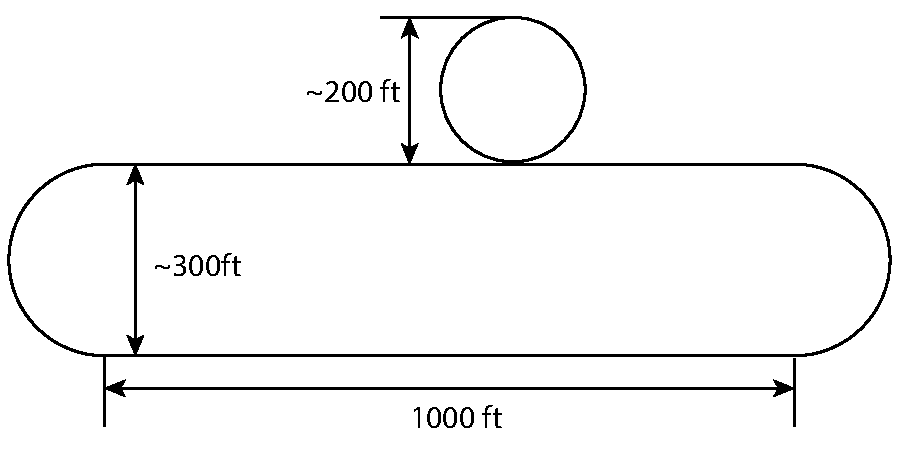
\includegraphics[width=4.5in]{coursedistances}
	\caption{This plot breaks down the estimated lengths of the course based on the scale drawing from the mission requirements.}
	\label{fig:course}
\end{figure}

%%%%%%%%%%%%%%%%%%%%%%%%%%%%%
%%%% - Sub-system Reqs - %%%%
%%%%%%%%%%%%%%%%%%%%%%%%%%%%%
\subsection{Sub-system Design Requirements}
\label{ssec:MissionReqs}

We have organized our sub-system requirements into aerodynamics, structure, propulsion, and specialty requirements explained below.

\subsubsection{Aerodynamics Requirements}
\label{sssec:AerodynamicReqs}

Some of the major requirements for the aerodynamics sub-system are: Maximize aerodynamic efficiency in order to use less energy to overcome drag for all flight missions.  Design wing loading to be able to take off and fly with design max payload weight.  Keep the wingspan within the maximum of {\color{BYUred}[MAX SPAN CONSTRAINT THIS YEAR]}.  Choose airfoil(s) and configuration that will make take off feasible in the {\color{BYUred}[THIS YEAR'S TAKE-OFF REQUIREMENT]}

\subsubsection{Structural Requirements}
\label{sssec:StructuralReqs}

The breakdown of mission requirements for the structures sub-system include: Minimize the structural weight while maintaining sufficient rigidity to keep the aerodynamics as designed, especially when full payload weight is in use.  Make sure the structure is sufficiently rigid to avoid aerodynamic flutter within the flight envelope. {\color{BYUred}[OTHER MISC. STRUCTURES REQUIREMENTS THIS YEAR (E.G. FOLDING WINGS.)]}

\subsubsection{Propulsion Requirements}
\label{sssec:PropulsionReqs}

The propulsion sub-system requirements are to: Have sufficient system efficiency and battery capacity to enable completion of the flight missions and maximizing speed with sufficient endurance while also providing sufficient thrust for {\color{BYUred}[THIS YEAR'S TAKE-OFF REQUIREMENT]}

\subsubsection{Specialty Requirements} %change this to be specifically what it is (like bomb drop or whatever the specific mission is)
\label{sssec:SpecialReqs}

{\color{BYUred}[REQUIREMENTS FOR THIS YEAR'S SPECIAL STUFF.]} 
\lipsum[2]




%%%%%%%%%%%%%%%%%%%%%%%%%%%%%%%
%%%% - Sensitivity Study - %%%%
%%%%%%%%%%%%%%%%%%%%%%%%%%%%%%%
\subsection{Scoring Sensitivity Analysis}
\label{ssec:SensitivityStudy}

%Figure related to sensitivity study, move around to get formatting correct...
\begin{figure}[h!]
	\centering
%	\raisebox{0pt}[\dimexpr\height-2\baselineskip\relax]{
		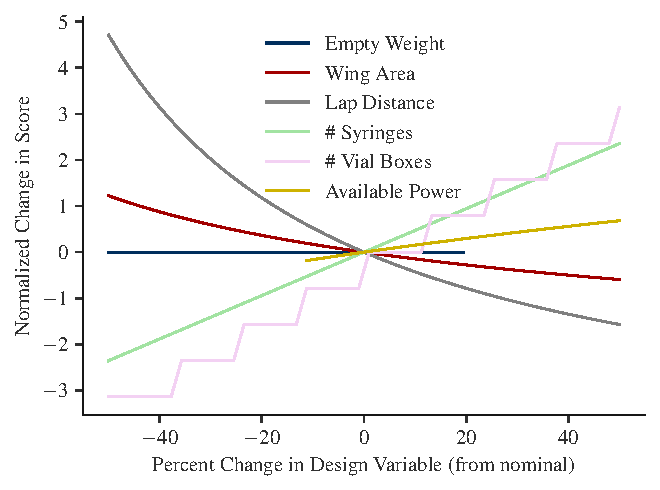
\includegraphics[]{sensitivityobj}
%	}
	\caption{This plot shows the effects of those design parameters that directly affect the increase/decrease in mission scoring beyond simple completion.}
	\label{fig:sensitivity}
\end{figure}

For our sensitivity study, we first differentiated between design variables that could increase/decrease our score and those that were only related to the minimum constraints. Furthermore, some aspects of the score are insensitive by design parameters, such as the design report score, the ground mission score, and the Flight Mission 1 score.  Our total, design-sensitive score is simply the sum of scores from Flight Mission 2 and 3.

{\color{\BYUred} [BREAKDOWN OF THE MATHS USED TO PERFORM THE SENSITIVITY STUDY.]}

In order to normalize the scores as they are in the competition, we ran the analysis first without normalization, from which we saved the maximum scores like they are in competition. We then used those maxima as the normalization factors and re-ran the analysis. This way we could simulate the competition normalizations for the scoring and one mission would not dominate another unrealistically.

In our analysis (results shown in \cref{fig:sensitivity}), we found that the wing area and parasitic drag coefficient induced negative sensitivities, thus we want to minimize drag and maximize wing loading (while still being able to take off).  The available power was also important, and can be affected by increasing battery capacity, discharge rate, or voltage, or increasing propulsive efficiency. {\color{BYUred}[TAKE AWAYS FROM PAYLOAD STUFF]}. We should also note that the aircraft weight had the lowest effect on the overall sensitivity, but is incredibly important to meeting the fixed constraints of the competition.




\subsection{Concept Review, Weighting, and Selection Process}
\label{ssec:selectionprocess}

Informed by our sensitivity study, \cref{tab:fom} shows our general figures of merit for our conceptual design choices. In addition to the primary mission sensitive parameters, we added some practical figures of merit as well.  In addition, rather than having multiple figures of the same value, we chose to make each figure a distinct value, thereby requiring a true prioritization and less change of ambiguity during the selection process.

We chose weight as the most important factor because it not only relates to the mission objectives, but also concerns the take-off/landing constraints.  Drag was our next highest factor, as speed is important for maximizing flight mission scores.  We placed simplicity next, as we must be able to actually produce our chosen design with our current and realistic potential abilities.  We found stability to be important as well, since our aircraft needs to be controllable if we are to compete, but stability is relatively easy to achieve for most designs, so it was given a relatively lower value to match.  Finally {\color{\BYUred}[TALK ABOUT THE YEAR SPECIFIC METRIC IF THERE IS ONE.]} Each of the decision matrices has additional figures of merit associated with sub-system specific requirements. Note also, that parameters associated with available power were not included in the general list of figures of merit, but are included in propulsion specific decision matrices.

%----------------
%---   Figure of Merit (i.e. the weights used in decision matrices)
%----------------
\begin{table}[h!]
	\centering
	\caption{Figures of Merit}
	\label{tab:fom}
	\rowcolors{2}{BYUbluelite}{white}
	\begin{tabular}{ c c } 

		\rowcolor{BYUbluemid}
		Factor & Scale (1-5) \\

		Weight & 10 \\

		Drag & 8 \\

		Simplicity & 6 \\

		Stability & 4 \\

		{\color{\BYUred} {\color{BYUred} [YEAR SPECIFIC ITEM]}} & 2 \\

	\end{tabular}
\end{table}


\subsubsection{Wing Configuration Selection}

For our wing configuration, we needed to take overall potential lift into account, due to the take-off/landing requirements.  \Cref{tab:wingconfiguration} shows our scoring for single wing, tandem wing, and bi/tri-wing configurations.  Note that we eliminated flying wing/blended wing body configurations up front based on our previous experience with that concept.

\lipsum[1]


%----------------
%---   Wing Configuration Decision Matrix (Convetional, Bi-Plane, Tandem Wing, etc.)
%----------------
\begin{table}[h!]
	\centering
	\caption{Weighted decision matrix for wing configuration.}
	\label{tab:wingconfiguration}
	\rowcolors{2}{white}{BYUbluelite}
	\begin{tabular}{ c c c c c } 

		\rowcolor{BYUbluemid}
    	\multicolumn{2}{c}{} & \parbox[c]{1in}{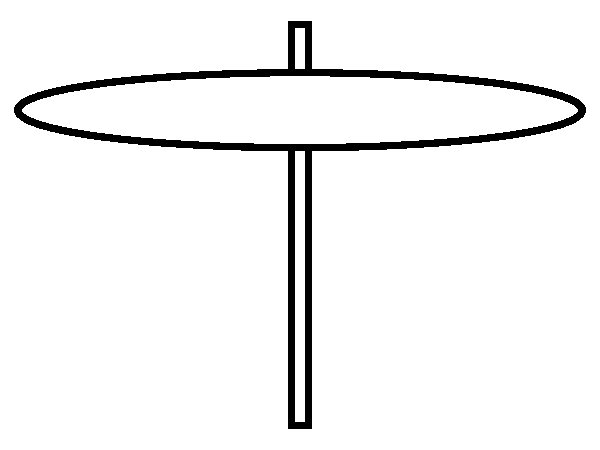
\includegraphics[width=1in]{singlewing}} & \parbox[c]{1in}{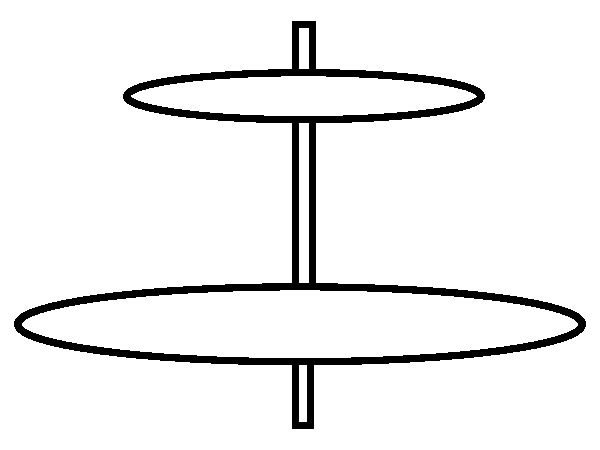
\includegraphics[width=1in]{tandemwing}} &  \parbox[c]{1in}{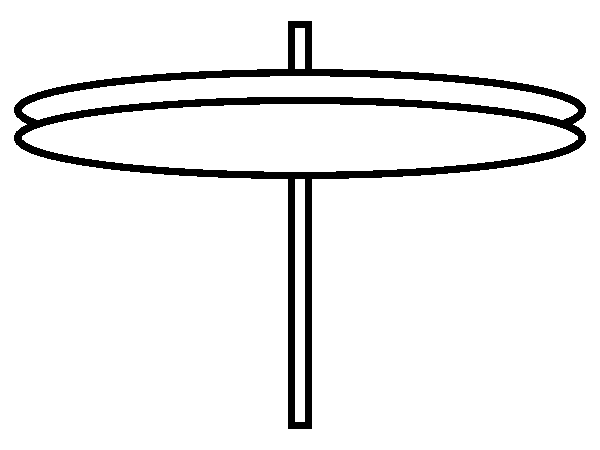
\includegraphics[width=1in]{biwing}} \\
    	
		\rowcolor{BYUbluemid} 
		Factor & Scale & Single Wing & Tandem Wing & Bi/Tri-wing \\
		
		Weight & 10 & 3 & 2 & 1 \\

		Drag & 8 & 3 & 2 & 1 \\

		Simplicity & 6 & 3 & 1 & 2 \\

		Lift & 5 & 2 & 2 & 3 \\

		Stability & 4 & 3 & 2 & 3 \\

		{\color{\BYUred} {\color{BYUred} [YEAR SPECIFIC ITEM]}} & 2 & & & \\

		\multicolumn{2}{c}{Totals} &  &  &  \\%BOLD WINNING OPTION

	\end{tabular}
\end{table}

\subsubsection{Wing Placement Selection}

For the wing placement, we compared high, mid, and low wing placement.  An addition figure of merit here is the accessibility, that is, the accessibility of the payload and electronics.  This is important not only for the ground mission, but also for setting up the aircraft for flight.

\lipsum[1]


%----------------
%---   Wing Placement Decision Matrix  (High, Mid, Low)
%----------------
\begin{table}[h!]
	\centering
	\caption{Weighted decision matrix for wing placement.}
	\label{tab:wingplacement}
	\rowcolors{2}{white}{BYUbluelite}
	\begin{tabular}{ c c c c c } 

		\rowcolor{BYUbluemid}
		& & High Wing & Mid Wing & Low Wing \\
		\rowcolor{BYUbluemid}
		Factor & Scale & \parbox[c]{1in}{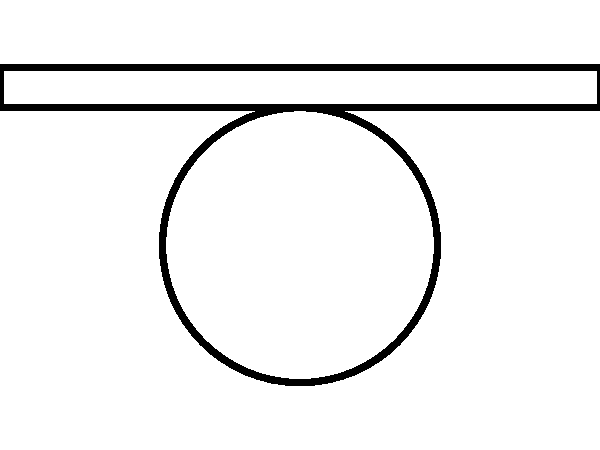
\includegraphics[width=1in]{highwing}} & \parbox[c]{1in}{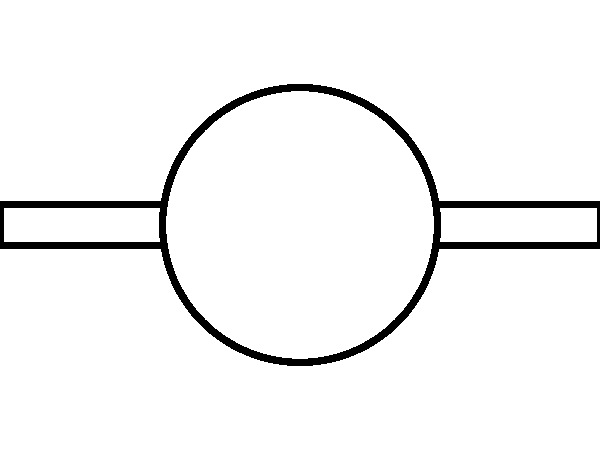
\includegraphics[width=1in]{midwing}} &  \parbox[c]{1in}{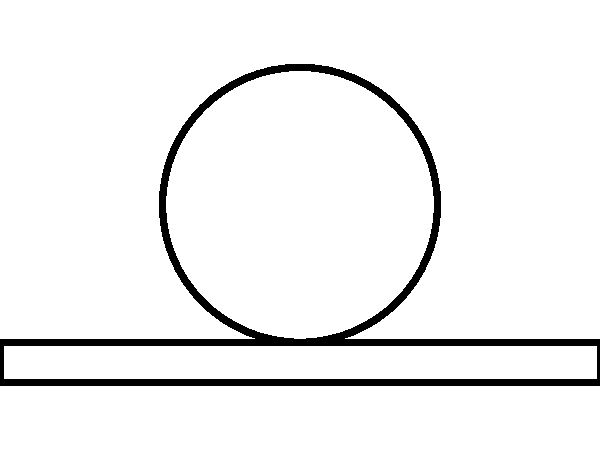
\includegraphics[width=1in]{lowwing}} \\

		Weight & 10 & 3 & 2 & 3 \\

		Drag & 8 & 2 & 3 & 2 \\

		Simplicity & 6 & 3 & 1 & 2 \\

		Accessibility & 5 & 1 & 2 & 3 \\

		Stability & 4 & 3 & 2 & 1 \\

		{\color{\BYUred} {\color{BYUred} [YEAR SPECIFIC ITEM]}} & 2 & & & \\

		\multicolumn{2}{c }{Totals} &  &  &  \\%BOLD WINNING OPTION

	\end{tabular}
\end{table}

\subsubsection{Empennage Configuration Selection}

For the tail configuration selection, we did not see the need for any further figures of merit.  We compared three families of configuration: T-tail family, including conventional, cruciform, and T-tail designs; V-tail family, including V- and inverted V-tail designs; and H-tail family, including U-, H-, and inverted U-tail designs.

\lipsum[1]


%----------------
%---  Tail Configuration Decision Matrix  (Conventional, H-tail, V-tail, Flying wing, etc.)
%----------------
\begin{table}[h!]
	\centering
	\caption{Weighted decision matrix for tail configuration.}
	\label{tab:tailconfiguration}
	\rowcolors{2}{white}{BYUbluelite}
	\begin{tabular}{ c c c c c } 

		\rowcolor{BYUbluemid}
		& & T-Tail Variations & V-Tail Variations & H-Tail Variations \\
		\rowcolor{BYUbluemid}
		Factor & Scale &
		\parbox[c]{1in}{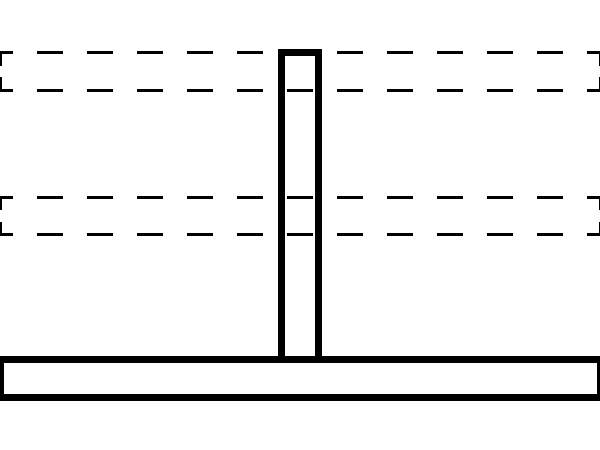
\includegraphics[width=1in]{ttail}} &
		\parbox[c]{1in}{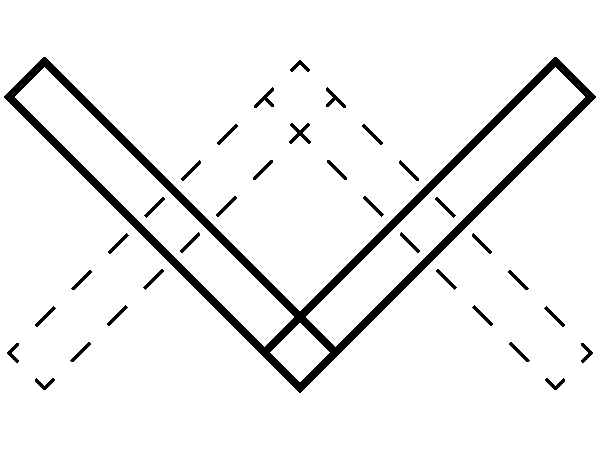
\includegraphics[width=1in]{vtail}} &
		\parbox[c]{1in}{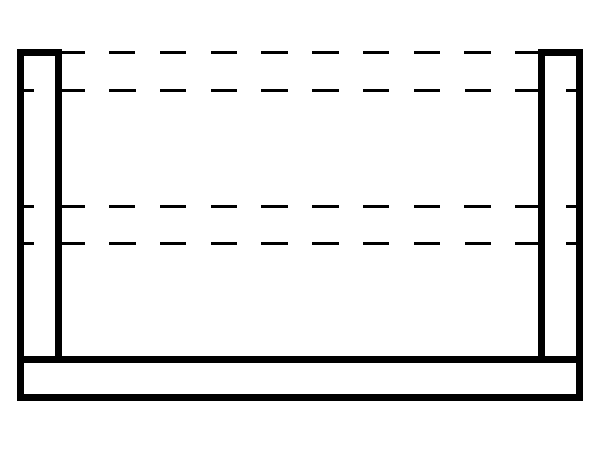
\includegraphics[width=1in]{htail}} \\

		Weight & 10 & 2 & 3 & 1 \\

		Drag & 8 & 2 & 3 & 2 \\

		Simplicity & 6 & 3 & 2 & 1 \\

		Stability & 4 & 2 & 1 & 3 \\

		{\color{\BYUred} {\color{BYUred} [YEAR SPECIFIC ITEM]}} & 2 & & & \\

		\multicolumn{2}{c }{Totals} &  &  &  \\%BOLD WINNING OPTION

	\end{tabular}
\end{table}


\subsubsection{Propulsion Configuration Selection}

For the propulsion configuration, drag did not make sense as a figure of merit, since the system is in direct opposition to drag.  Therefore we exchanged drag for efficiency, since efficiency directly affects available power (which we found to be important in \cref{ssec:SensitivityStudy}).  We also included lift as a figure of merit for the propulsion system, because blown wing configurations can experience increased lift (due to higher induced velocities over the wing).

\lipsum[1]


%----------------
%---   Propulsion Configuration Decision Matrix  (single prop, dual prop, distributed propulsion, etc.)
%----------------
\begin{table}[h!]
	\centering
	\caption{Weighted decision matrix for propulsion configuration.}
	\label{tab:propconfiguration}
	\rowcolors{2}{white}{BYUbluelite}
	\begin{tabular}{ c c c c c } 

		\rowcolor{BYUbluemid}
		& & Single Prop & Dual Prop & Distributed Prop \\
		\rowcolor{BYUbluemid}
		Factor & Scale & \parbox[c]{1in}{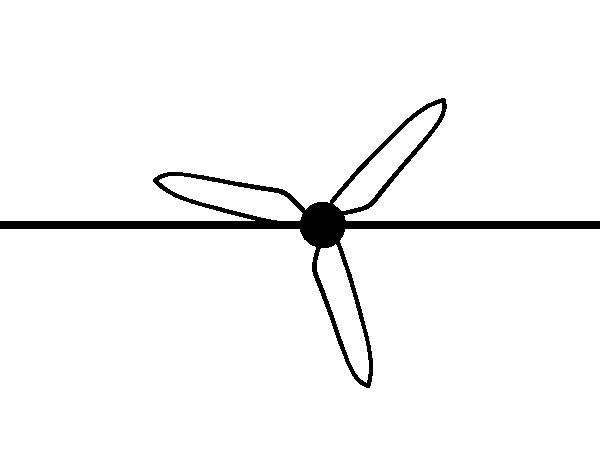
\includegraphics[width=1in]{singleprop}} & \parbox[c]{1in}{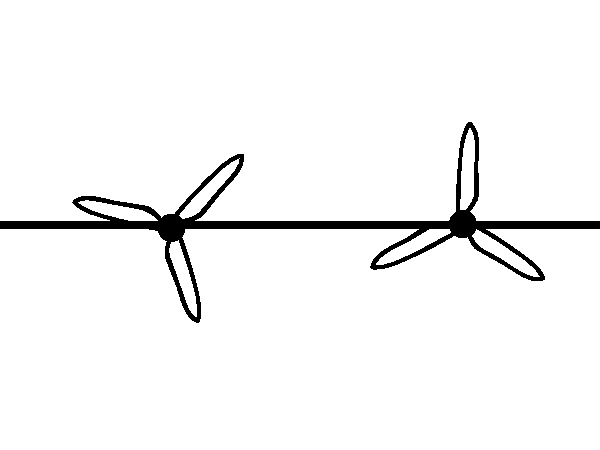
\includegraphics[width=1in]{dualprop}} &  \parbox[c]{1in}{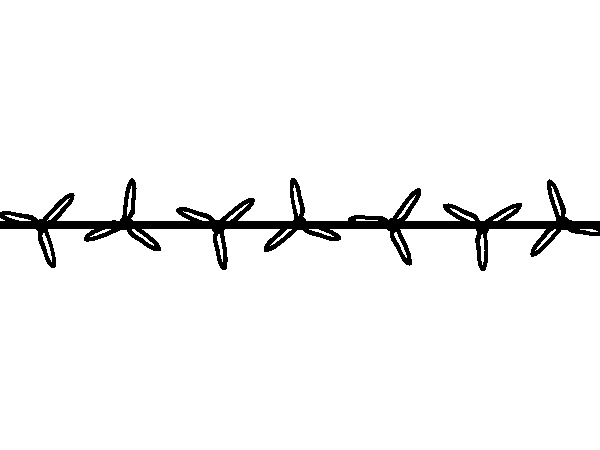
\includegraphics[width=1in]{distributedprop}} \\

		Weight & 10 & 3 & 2 & 1 \\

		Propulsive Efficiency & 8 & 1 & 2 & 3 \\

		Lift & 7 & 1 & 2 & 3 \\

		Simplicity & 6 & 3 & 2 & 1 \\

		Stability & 4 & 3 & 2 & 3 \\

		{\color{\BYUred} {\color{BYUred} [YEAR SPECIFIC ITEM]}} & 2 & & & \\

		\multicolumn{2}{c }{Totals} &  &  &  \\%BOLD WINNING OPTION

	\end{tabular}
\end{table}

\subsubsection{Propulsion Placement Selection}



\lipsum[1]


%----------------
%---   Propulsion Placement Decision Matrix  (tractor, pusher, etc)
%----------------
\begin{table}[h!]
	\centering
	\caption{Weighted decision matrix for propulsion placement.}
	\label{tab:propplacement}
	\rowcolors{2}{white}{BYUbluelite}
	\begin{tabular}{ c c c c c } 

		\rowcolor{BYUbluemid}
		& & Pull Variations & Push Variations & Combinations \\
		\rowcolor{BYUbluemid}
		Factor & Scale & 
		\parbox[c]{1in}{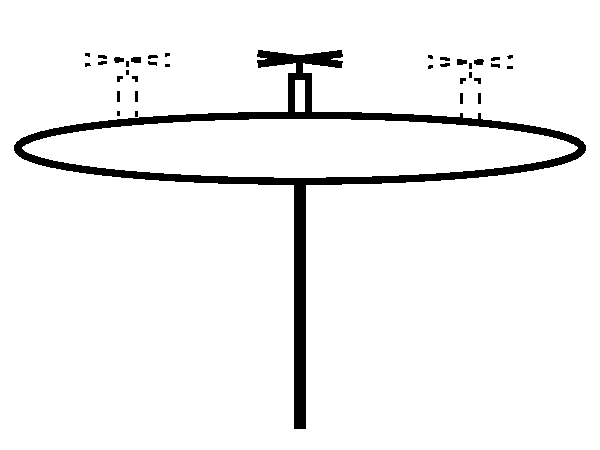
\includegraphics[width=1in]{puller}} &
		\parbox[c]{1in}{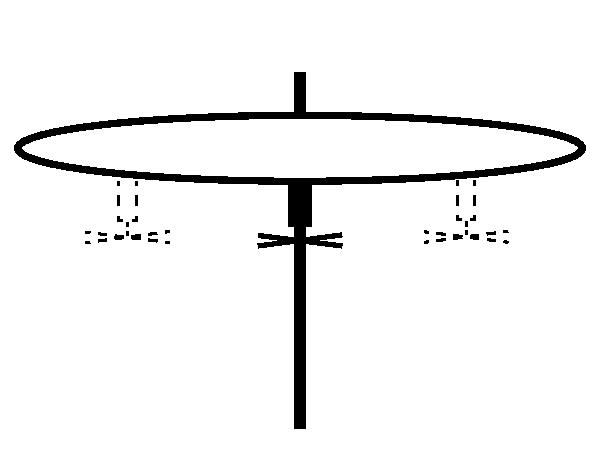
\includegraphics[width=1in]{pusher}} &
		\parbox[c]{1in}{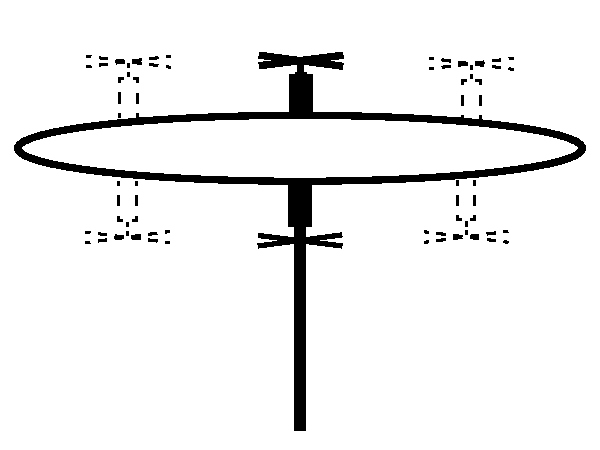
\includegraphics[width=1in]{combopushpull}} \\

		Weight & 10 & 3 & 3 & 3 \\

		Lift & 4 & 3 & 1 & 2 \\

		Simplicity & 6 & 3 & 2 & 1 \\

		Propulsive Efficiency & 4 & 3 & 1 & 2 \\

		{\color{\BYUred} {\color{BYUred} [YEAR SPECIFIC ITEM]}} & 2 & & & \\

		\multicolumn{2}{c }{Totals} &  &  &  \\%BOLD WINNING OPTION

	\end{tabular}
\end{table}

\subsubsection{Payload}
\label{sssec:payloadconcept}

\lipsum[1]


%----------------
%---   Payload Decision Matrix.
%----------------
\begin{table}[h!]
	\centering
	\caption{Weighted decision matrix for {\color{\BYUred} [SPECIFY THIS YEAR'S PAYLOAD DESIGN]}.}
	\label{tab:payloadconfiguration}
	\rowcolors{2}{white}{BYUbluelite}
	\begin{tabular}{ c c c c c } 

		\rowcolor{BYUbluemid}
		& & {\color{BYUred} [OPTION]} & {\color{BYUred} [OPTION]} & {\color{BYUred} [OPTION]} \\
		\rowcolor{BYUbluemid}
		Factor & Scale & \parbox[c]{1in}{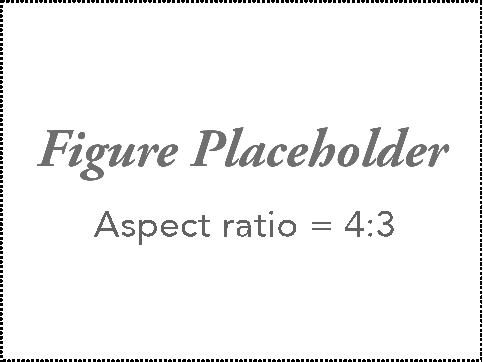
\includegraphics[width=1in]{draft4x3}} & \parbox[c]{1in}{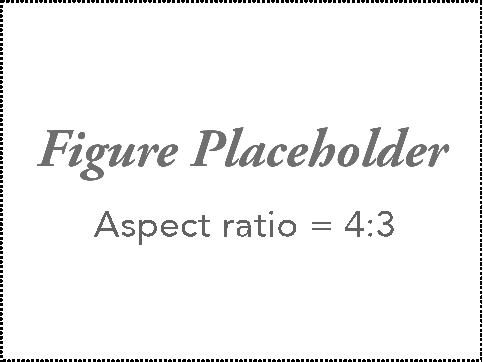
\includegraphics[width=1in]{draft4x3}} &  \parbox[c]{1in}{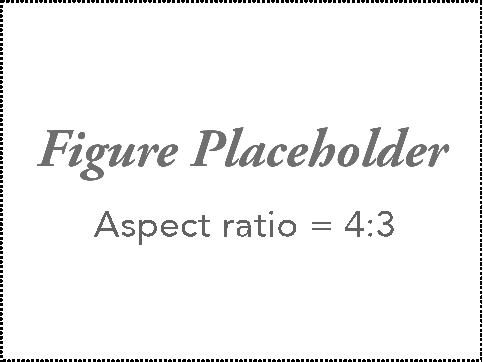
\includegraphics[width=1in]{draft4x3}} \\

		Weight & 10 & & &\\

		Strength & 8 & & & \\

		Simplicity & 6 & & & \\

		Durability & 4 & & & \\

		{\color{\BYUred} {\color{BYUred} [YEAR SPECIFIC ITEM]}} & 2 & & & \\

		\multicolumn{2}{c }{Totals} &  &  &  \\%BOLD WINNING OPTION

	\end{tabular}
\end{table}


\lipsum[1]


\subsubsection{Final Concept}
\label{sssec:finalconcept}

\lipsum[1]

%----------------
%---  Figure of the final concept
%----------------
\begin{figure}[h!]
	\centering
	\begin{subfigure}[b]{0.475\textwidth}
		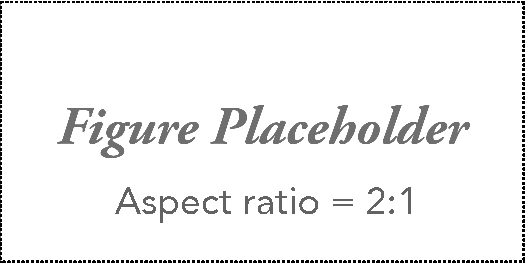
\includegraphics[width=\textwidth]{draft2x1}
		\caption{Top View}
		\label{fig:topview}
	\end{subfigure}
	%
	\begin{subfigure}[b]{0.475\textwidth}
		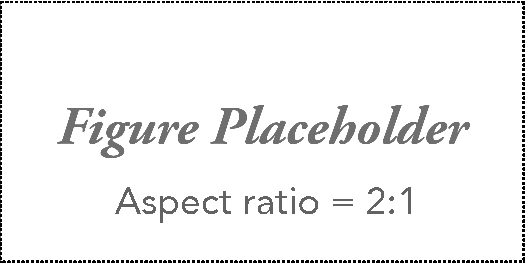
\includegraphics[width=\textwidth]{draft2x1}
		\caption{Side View}
		\label{fig:sideview}
	\end{subfigure}
	
	\begin{subfigure}[b]{0.475\textwidth}
		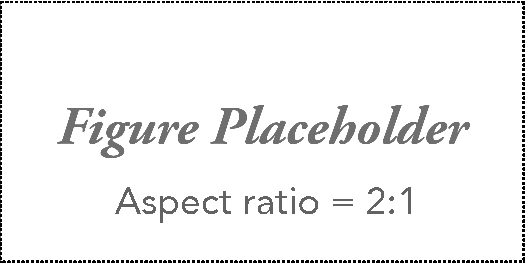
\includegraphics[width=\textwidth]{draft2x1}
		\caption{Front View}
		\label{fig:frontview}
	\end{subfigure}
	%
	\begin{subfigure}[b]{0.475\textwidth}
		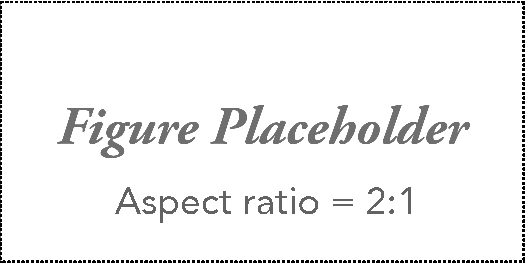
\includegraphics[width=\textwidth]{draft2x1}
		\caption{Rendered View}
		\label{fig:renderedview}
	\end{subfigure}
	\caption{Drawings and rendering of our conceptual aircraft design.}
	\label{fig:prelimdrawings}
\end{figure}